\documentclass[conference]{IEEEtran}
\IEEEoverridecommandlockouts
\usepackage{cite}
\usepackage{amsmath,amssymb,amsfonts}
\usepackage{algorithmic}
\usepackage{graphicx}
\usepackage{booktabs}
\usepackage{textcomp}
\usepackage{xcolor}
\usepackage{hyperref}
\usepackage{url}
\def\BibTeX{{\rm B\kern-.05em{\sc i\kern-.025em b}\kern-.08em
    T\kern-.1667em\lower.7ex\hbox{E}\kern-.125emX}}
\begin{document}

\title{Credit card fraud detection using a clustering approach\\
}

\author{\IEEEauthorblockN{María Camila Vásquez Correa}
\IEEEauthorblockA{\textit{Mathematics department} \\
\textit{Universidad EAFIT}\\
Medellín, Colombia \\
mvasqu49@eafit.edu.co}
}

\maketitle

\begin{abstract}
In this article is presented a comparison of 5 clustering algorithms to segregate data on credit card fraud detection, these algorithms are: k-means, an extension to k-means, fuzzy c-means, subtractive and mountain clustering. These algorithms are first evaluated in the iris dataset, and finally in our case study. Several metrics for finding the clusters are compared and a variation of parameters is performed.
\end{abstract}

\begin{IEEEkeywords}
Cluster, k-means, credit card, fraud.
\end{IEEEkeywords}

\section{Introduction}
Given the current global economic
context, increasing efforts are being made to both prevent and detect fraud. Credit card financial products can derive in unsecured and unplanned credit card risks and should not be underestimated. Stopping credit card fraud has become a hot issue in academia and industry. In the field of credit card fraud, the mistake of letting go of fraudulent transactions is much more expensive than mistakenly intercepting normal transactions, and the number of fraudulent transactions is far less than the normal number of transactions. \\
Clustering, as unsupervised data mining technique, deals with the problem of dividing a given set of entities into meaningful subsets. Clusters resulted from this data segmentation are required to be to be homogeneous and/or well separated, entities within the same group being similar while entities within different groups being dissimilar. 

\section{Literature review}
A survey for the methods on fraud detection via clustering is presented in\cite{Sabau2012}. This survey takes into account the algorithm used and the type of fraud the models are attacking. Is clear that the prevalent method is the k-means, however, some other types of clustering including graph based, hierarchical and density based algorithms were also implemented in the reviewed works. \\
As an example, some of the methods that make good use of the k-means clustering are: \cite{Wang2019a}, who compares the performance of Support Vector Machines along with clustering algorithms and other classification approaches, and finds put that the former is better at handling highly unbalanced data. \cite{Santos2018} uses a Naive Bayes clustering approach (as well as \cite{Carneiro2015a}) along with k-means clustering. In these algorithms, there is a clear pattern of hybrid methodologies, some other examples include \cite{Sathyapriya2019}, \cite{Kumari2017}, and \cite{Fashoto2016a} that use Hidden Markov models along with k-means clustering with the objective of reducing the false alarms produced by other algorithms of fraud detection and to include information about past transactions to build a costumer profile. However, some authors like \cite{Carneiro2015a} use only Naive Bayes clustering along with a Multi Layer perceptron to build a clustering engine and \cite{Behera2015a} makes use of fuzzy c-means clustering and builds stochastic models along with artificial neural networks to achieve the same objectives. Finally, hierarchical clustering paired with classification techniques is also useful, as shown in \cite{Wang2018}. \\
In this work we aim to use only clustering techniques to analyze a dataset containing some fraudulent transactions and the features associated with them. These clustering techniques will be analyzed in order to get some insights about the data and the costumers.

\section{Methodology}

\subsection{Data}
\begin{enumerate}
    \item \textit{Toy dataset: }The initial test dataset for the algorithms was the iris dataset, that contains 3 classes of iris flowers (versicolor, virginica and setosa) and has 4 features (sepal length and height and petal length and width) with 150 samples.
    \item \textit{Credit card dataset: } This dataset was downloaded from Kaggle (\url{https://www.kaggle.com/mlg-ulb/creditcardfraud}) and contains transactions made by credit cards in September 2013 by european cardholders. This dataset presents transactions that occurred in two days, where we have 492 frauds out of 284,807 transactions. The dataset is highly unbalanced, the positive class (frauds) account for 0.172\% of all transactions.
\end{enumerate}

\subsection{Pipeline}
\begin{enumerate}
    \item \textit{Preprocessing: }Elimination of missing values and normalization. The normalization method performed is dividing by the maximum of each feature. This to ensure that all the data points are mapped into the hypercube [0,1].
    \item \textit{Statistical analysis:} In order to asses the complexity of the problem, several statistical tests were taken, including normality tests, Independence tests, dsitribution tests and stationarity tests. 
    \item \textit{Feature selection and extraction: }This step was performed differently in both datasets, the toy dataset and the credit card dataset. In the first one, 4 characteristics were extracted, augmenting the dimension from 4 to 8. In the second one, 28 characteristics were provided, and a reduction of dimensionality via PCA was performed.
    \item \textit{Embbeding: }The T-distributed Stochastic Neighbor Embedding was used as embbeding algorithm, due to its distance conserving property. This embbeding was used to visualize the results and also to learn in lower dimensions.
    \item \textit{Learning: }5 clustering algorithms were implemented in both datasets, performing the learning task in the higher, medium and lower dimensional space and comparing the results.
\end{enumerate}
\subsection{Algorithms}
Let $\{x_1,\dots,x_n\}$ be $n$ data points in an $M$ dimensional space, normalized to an hypercube. Also, let $d(x,y)$ be a distance function in $\mathbb{R}^n$.
\begin{enumerate}
    \item \textit{Subtractive clustering:} This method takes all the points as cluster centers candidates. The steps for the algorithm are:
    \begin{enumerate}
        \item Calculate a density function for each pint $x_i$, given by:
    \begin{equation*}
        D_i = \sum_{i=1}^n \exp\left(-\frac{d(x_i,x_j)^2}{(r_a/2)^2}\right)
    \end{equation*}
    where $r_a$ is a positive constant representing a neighborhood radius. 
    \item Choose the cluster center $x_{ci}$ as the point having the largest density value $D_{c_i}$. 
    \item Revise each point's density function by eliminating the effect of the previously chosen center as follows:
\begin{equation*}
    D_i = D_i - D_{c_i}\exp\left(-\frac{d(x_i,x_{c_i})^2}{(r_b/2)^2}\right)
\end{equation*}
where $r_b$ is a positive constant which defines a neighborhood that has measurable reductions in density measure.
\item If a sufficient number of clusters is reached, or the value of the density function is too small, stop. If not, go back to step 2.
    \end{enumerate}
    \item \textit{Mountain clustering:}
    This method, instead of taking each point as a cluster candidate, it forms a grid in the data space, where the intersections of the grid lines represent the potential cluster centers. These points are stored in set $V$. Then, we apply the following algorithm:
    \begin{enumerate}
        \item Calculate a mountain function for each point $v_j$ in $V$, given by:
    \begin{equation*}
        m_j = \sum_{i=1}^n \exp\left(-\frac{d(v_j-x_i)^2}{2\sigma^2}\right)
    \end{equation*}
    where $\sigma$ is a positive constant representing the height and the smoothness of the mountain. 
    \item Choose the cluster center $v_{ci}$ as the point having the largest mountain value $m_{c_i}$. 
    \item Revise each point's mountain function by eliminating the effect of the previously chosen center as follows:
\begin{equation*}
    m_j = m_j - m_{c_i}\exp\left(-\frac{d(v_j-v_{c_i})^2}{(2\beta^2}\right)
\end{equation*}
where $\beta$ is a positive constant.
\item If a sufficient number of clusters is reached, or the value of the mountain function is too small, stop. If not, go back to step 2.
    \end{enumerate}
    \item \textit{k-means clustering} In this algorithm, the dataset is going to be partitioned in $k$ groups $G_i$, $i = 1,\dots,k$. The cost function, based on a distance $d(x,y)$, can be defined by:
    \begin{equation*}
        J = \sum_{i=1}^c J_i = \sum_{i=1}^c\left(\sum_{k,x_k\in G_i} d(x_k,c_i)^2\right)
    \end{equation*}
    For the development, we follow these steps:
    \begin{enumerate}
        \item Randomly initialize the cluster centers $c_i$, $i = 1,\dots, k$.
        \item Determine a membership matrix for each group, $U$ by:
        \begin{equation*}
            u_{ij} = \left\lbrace\begin{array}{ll}
            1     & ||x_j - c_i||^2 \leq ||x_j - c_k||^2 \qquad \forall k\neq i \\
             0    & \text{ Otherwise} 
            \end{array}\right.
        \end{equation*}
        \item Compute the cost function. Stop if it is bellow a certain tolerance $\varepsilon$ or its improvement is irrelevant.
        \item Update the cluster centers by:
        \begin{equation*}
            c_i = \frac{1}{|G_i|}\sum_{k, x_k\in G_i}x_k
        \end{equation*}
        Then, go to the second step.
    \end{enumerate}
    \item \textit{Fuzzy c-means clustering}
    In this algorithm, each point of the dataset belongs to each of the $c$ clusters in a certain degree of membership, between 0 and 1. The steps to follow are:
    \begin{enumerate}
        \item Initialize the membership matrix $U$ with random values between 0 and 1 such that:
        \begin{equation*}
            \sum_{i=1}^c u_{ij} = 1 \qquad \forall j=1,\dots, n
        \end{equation*}
        \item Calculate $c$ fuzzy cluster centers $c_i$, $i = 1,\dots,n$ by:
        \begin{equation*}
            c_i = \frac{\sum_{j=1}^n u_{ij}^m x_j}{\sum_{j=1}^n u_{ij}^m}
        \end{equation*}
        \item Compute the cost function:
        \begin{equation*}
            J(U,c_1,\dots,c_c) = \sum_{i=1}^cJ_i = \sum_{i=1}^c\sum_{j=1}^n u_{ij}^md_{ij}^2
        \end{equation*}
        where $u_{ij}$ is between 0 and 1, $c_i$ is the cluster center of fuzzy group $i$, $d_{ij} = d(c_i,x_j)$ and $m\in[1,\infty)$ is a weighting exponent. Stop if it is either bellow a certain tolerance $\varepsilon$ or if there is no improvement.
        \item Compute a new membership matrix using the following:
        \begin{equation*}
            u_{ij} = \frac{1}{\sum_{k=1}^c\left(\frac{d_{ij}}{d_{kj}}\right)^{\frac{2}{m-1}}}
        \end{equation*}
        Then, go to step 2.
    \end{enumerate}
    \item \textit{K-medians clustering} This is a variation of the k-means clustering \cite{median} in which, instead of computing the mean of the points in a cluster, one calculates the median. This algorithm is more robust to outliers in the dataset.
\end{enumerate}
\subsection{Distance functions}
As defined above, all of the mentioned algorithms calculate distances between points. Let $x = (x_1,\dots,x_n)$ and $y = (y_1,\dots,y_n)$ be two points in $\mathbb{}^n$. The distance functions that are going to be used are the following:
\begin{itemize}
    \item \textit{Euclidean distance}
    \begin{equation*}
        d(x,y) = \sqrt{\sum_{i=1}^n (x_i-y_i)^2}
    \end{equation*}
    \item \textit{Manhattan distance}
    \begin{equation*}
       d(x,y)  = \sum_{i=1}^n |x_i-y_i|
    \end{equation*}
    \item \textit{Cosine similarity}
    \begin{equation*}
        d(x,y) = \frac{\sum_{i=1}^n x_iy_i}{\sum_{i=1}^n x_i^2\sum_{i=1}^n y_i^2}
    \end{equation*}
\end{itemize}
\subsection{Validation}
Both datasets contain groundtruths for the classes of each sample. The previously presented algorithms will be evaluated using some indices (intra cluster and extra cluster) with both of the datasets. Let $c_i$, $i = 1,\dots, k$ be the cluster centers and $C_i$ be the sets containing the points of each cluster. The indices used are described in \cite{validation} and include:
\begin{itemize}
    \item \textit{Davies-Bouldin (DB) index} This index us a function of the \textit{within cluster scatter} and the \textit{between cluster separation}. We define:
    \begin{enumerate}
        \item Within cluster scatter: $S_i = \displaystyle{\frac{1}{|C_i|}\sum_{x\in C_i}||x - z_i||}$.
        \item Between cluster separation: Is simply the distance $d_{ij}$ between two cluster centers $||c_i-c_j||$.
        \item $\displaystyle{R_{i,qt} = \max\limits_{j,j\neq i}\left\lbrace\frac{S_{i,q} + S_{j+q}}{d_{ij}t}\right\rbrace}$
    \end{enumerate}
    And the index is defined as:
    \begin{equation*}
        DB = \frac{1}{k}\sum_{i=1}^k R_{i,qt}
    \end{equation*}
    The objective is to minimize this index for proper clustering.
    \item \textit{Calinski Harabasz (CH) Index} Let $c$ be the centroid of the entire dataset. The index is defined as
    \begin{equation*}
        CH = \frac{ \left[\frac{\sum_{l = 1}^k |C_l|||c_l - c||^2}{k-1}\right]}{\left[\frac{\sum_{l=1}^k \sum_{i=1}^{|C_l}||x_i-c_l||^2}{n-k}\right]}
    \end{equation*}
\end{itemize}

\section{Results}
\subsection{Iris dataset}

\begin{itemize}
    \item \textbf{Subtractive clustering}\\
    The iris dataset contains a ground truth of 3 clusters. In Tables \ref{tab:i1_n_s}, \ref{tab:i2_n_s} and \ref{tab:ie_n_s} are described the number of clusters found by the subtractive algorithm with various configurations of neighborhood ratios $r_a$ and metrics. The Figures \ref{fig:sub-i-iris} and \ref{fig:sub-f-iris} show the initial state of the density function and the final state for one configuration ($r_a =0.5$, metric euclidean),respectively.
    \begin{table}[ht!]
        \centering
        \begin{tabular}{lrrr}
        \toprule
        $r_a$ &  euclidean &  cosine &  cityblock \\
        \midrule
        0.4 &          4 &       1 &          6 \\
        0.5 &          3 &       1 &          4 \\
        0.7 &          2 &       1 &          3 \\
        \bottomrule \\
\end{tabular}
        \caption{Number of clusters given by the subtractive cluster for the iris dataset.}
        \label{tab:i1_n_s}
    \end{table}
    \begin{table}[ht!]
        \centering
        \begin{tabular}{lrrr}
        \toprule
        $r_a$ &  euclidean &  cosine &  cityblock \\
        \midrule
        0.4 &         99 &       4 &         99 \\
        0.5 &         93 &       4 &         99 \\
        0.7 &          8 &       3 &         94 \\
        \bottomrule \\
        \end{tabular}
        \caption{Number of clusters given by the subtractive cluster for the augmented iris dataset.}
        \label{tab:i2_n_s}
    \end{table}
    
    \begin{table}[ht!]
        \centering
        \begin{tabular}{lrrr}
        \toprule
        $r_a$ &  euclidean &  cosine &  cityblock \\
        \midrule
        0.4 &         99 &       3 &         99 \\
        0.5 &         91 &       2 &         99 \\
        0.7 &         37 &       2 &         48 \\
        \bottomrule \\
        \end{tabular}
        \caption{Number of clusters given by the subtractive cluster for the embbeded iris dataset.}
        \label{tab:ie_n_s}
    \end{table}
    Despite the fact that the dataset provides clearly at least 2 groups, the results vary among the different parameters for the subtractive algorithm. We observe that, for the embbeded data, the cosine norm is usually better than the others, as well as for the augmented dataset. But the euclidean norm works better for the original dataset, as shown in Figure~\ref{fig:sub-iris}.
    \begin{table}[ht!]
        \centering
        \begin{tabular}{lrrr}
        \toprule
        $r_a$ &   euclidean &  cosine &   cityblock \\
        \midrule
        0.4 &  523.017618 &     NaN &  415.515675 \\
        0.5 &  603.592099 &     NaN &  522.011796 \\
        0.7 &  497.999891 &     NaN &  594.486176 \\
        \bottomrule \\
        \end{tabular}
        \caption{Calinski-Harabasz score for the iris dataset clustered with the subtractive algorithm.}
        \label{tab:i1_ch}
    \end{table}
    \begin{table}[ht!]
        \centering
        \begin{tabular}{lrrr}
        \toprule
        $r_a$ &  euclidean &  cosine &  cityblock \\
        \midrule
        0.4 &   0.800206 &     NaN &   1.054853 \\
        0.5 &   0.634911 &     NaN &   0.817205 \\
        0.7 &   0.390944 &     NaN &   0.640144 \\
        \bottomrule \\
        \end{tabular}
        \caption{Davies-Bouldin index for the iris dataset clustered with the subtractive algorithm.}
        \label{tab:i1_db}
    \end{table}
    In Tables \ref{tab:i1_ch} and \ref{tab:i1_db} we observe two indices for the clustering performed in the original dataset. Note that, for the cosine norm the number of clusters achieved is 1, and the metric is not defined for less than 2 groups. We can observe that the highest score and the lowest index are achieved with the euclidean norm, as we stated in the results for the number of clusters.
    \begin{table}[ht!]
        \centering
        \begin{tabular}{lrrr}
        \toprule
        $r_a$ &     euclidean &    cosine &     cityblock \\
        \midrule
        0.4 &  76625.576579 &  3.018177 &  78208.081628 \\
        0.5 &  53652.621959 &  3.874866 &  74559.857679 \\
        0.7 &      2.602149 &  4.132075 &  55651.428403 \\
        \bottomrule \\
        \end{tabular}
        \caption{Calinski-Harabasz score for the augmented iris dataset clustered with the subtractive algorithm.}
        \label{tab:i2_cb}
    \end{table}
    \begin{table}[ht!]
        \centering
        \begin{tabular}{lrrr}
        \toprule
        $r_a$ &  euclidean &    cosine &  cityblock \\
        \midrule
        0.4 &   0.217657 &  1.903561 &   0.219811 \\
        0.5 &   0.221893 &  1.861367 &   0.228289 \\
        0.7 &   2.739684 &  1.963818 &   0.258687 \\
        \bottomrule \\
        \end{tabular}
        \caption{Davies-Bouldin index for the augmented iris dataset clustered with the subtractive algorithm.}
        \label{tab:i2_db}
    \end{table}
    In Tables \ref{tab:i2_cb} and \ref{tab:i2_db} are shown the results for the validation on the augmented dataset. As seen before, the cosine norm achieves an appropiate number of clusters for this dataset, however, its indices and scores are the worst performed, probably because the other metrics achieve clusters that, even when they are not much informative, separate well the data and overfits the score. \\ 
    \begin{table}[ht!]
        \centering
        \begin{tabular}{lrrr}
        \toprule
        $r_a$ &    euclidean &       cosine &    cityblock \\
        \midrule
        0.4 &  9150.473726 &  2055.146690 &  8762.051647 \\
        0.5 &  6450.492142 &  1626.713464 &  8176.198965 \\
        0.7 &  3367.100226 &  1626.713464 &  3643.894411 \\
        \bottomrule \\
        \end{tabular}
        \caption{Calinski-Harabasz score for the embbeded iris dataset clustered with the subtractive algorithm.}
        \label{tab:ie_ch}
    \end{table}
    \begin{table}[ht!]
        \centering
        \begin{tabular}{lrrr}
        \toprule
        $r_a$ &  euclidean &    cosine &  cityblock \\
        \midrule
        0.4 &   0.270312 &  0.423202 &   0.279279 \\
        0.5 &   0.327560 &  0.216722 &   0.290310 \\
        0.7 &   0.626248 &  0.216722 &   0.564174 \\
        \bottomrule \\
        \end{tabular}
        \caption{Davies-Bouldin index for the embbeded iris dataset clustered with the subtractive algorithm.}
        \label{tab:ie_db}
    \end{table}
    \ \\
    Finally, in Tables \ref{tab:ie_db} and \ref{tab:ie_ch} we observe the valdiation results for the embbeded dataset (that contained only 2 features). Again, as for the augmented dataset, the euclidean and cityblock metrics are performing better, but we observe that is probably because the number of clusters achieved is huge.
    \begin{figure}[ht]
    \centering
    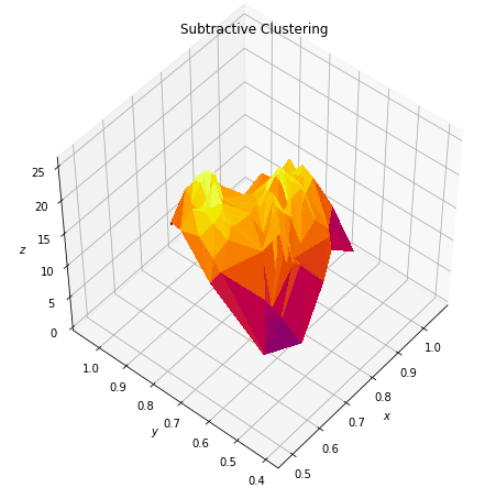
\includegraphics[scale = 0.45]{figures/iris/subtractive-i.png}
    \caption{Initial density function for the subtractive clustering using the euclidean norm.}
    \label{fig:sub-i-iris}
\end{figure}

\begin{figure}[ht]
    \centering
    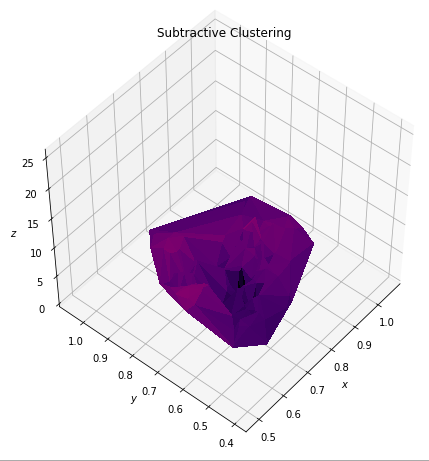
\includegraphics[scale = 0.5]{figures/iris/subtractive-f.png}
    \caption{Final density function for the subtractive clustering using the euclidean norm.}
    \label{fig:sub-f-iris}
\end{figure}

\begin{figure}[ht]
    \centering
    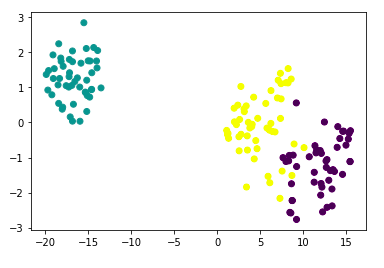
\includegraphics[scale = 0.5]{figures/iris/subtractive.png}
    \caption{Clustering for the iris dataset using the subtractive algorithm.}
    \label{fig:sub-iris}
\end{figure}

    \item \textbf{Mountain clustering:}
     In Tables \ref{tab:i1_n_m}, \ref{tab:i2_n_m} and \ref{tab:ie_n_m} are described the number of clusters found by the mountain algorithm with various configurations of smoothing parameters $\sigma$ and metrics. For $\sigma = 1.5$ and the euclidean metric, the first and last mountain function is shown in Figures \ref{fig:mon-i-iris} and \ref{fig:sub-f-iris}, respectively.
    \begin{table}[ht!]
        \centering
        \begin{tabular}{lrrr}
            \toprule
            $\sigma$ &  euclidean &  cosine &  cityblock \\
            \midrule
            0.4 &          5 &       3 &          7 \\
            0.5 &          3 &       2 &          4 \\
            0.7 &          2 &       1 &          3 \\
            \bottomrule \\
        \end{tabular}
        \caption{Number of clusters found by the mountain algorithm in the iris dataset.}
        \label{tab:i1_n_m}
    \end{table}
    
    \begin{table}[ht!]
        \centering
        \begin{tabular}{lrrr}
        \toprule
        $\sigma$ &  euclidean &  cosine &  cityblock \\
        \midrule
        0.4 &          4 &       4 &          2 \\
        0.5 &          3 &       4 &          2 \\
        0.7 &          2 &       2 &          2 \\
        \bottomrule \\
        \end{tabular}
        \caption{Number of clusters found by the mountain algorithm in the augmented iris dataset.}
        \label{tab:i2_n_m}
    \end{table}
    
    \begin{table}[ht!]
        \centering
        \begin{tabular}{lrrr}
        \toprule
        $\sigma$ &  euclidean &  cosine &  cityblock \\
        \midrule
        0.4 &          2 &       3 &          2 \\
        0.5 &          2 &       3 &          2 \\
        0.7 &          3 &       2 &          3 \\
        \bottomrule \\
        \end{tabular}
        \caption{Number of clusters found by the mountain algorithm in the embbeded iris dataset.}
        \label{tab:ie_n_m}
    \end{table}
    In comparison with the subtractive algorithm, the mountain algorithm is able to approximate better the number of clusters existing in the iris dataset, for any configuration of the smoothing parameter $\sigma$ and metric. However, as shown in the results of Figure~\ref{fig:mon-iris}, some configurations are better than others in finding the correct amount of clusters.
    \begin{table}[ht!]
        \centering
        \begin{tabular}{lrrr}
        \toprule
        $\sigma$ &   euclidean &  cosine &   cityblock \\
        \midrule
        0.4 &  392.333739 &     NaN &  245.874313 \\
        0.5 &  586.577476 &     NaN &  419.084383 \\
        0.7 &  497.999891 &     NaN &  567.385797 \\
        \bottomrule \\
        \end{tabular}
        \caption{Calinski-Harabasz score for the iris dataset clusterd by the mountain algorithm.}
        \label{tab:i1_ch_m}
    \end{table}
    
    \begin{table}[ht!]
        \centering
        \begin{tabular}{lrrr}
        \toprule
        $\sigma$ &  euclidean &  cosine &  cityblock \\
        \midrule
        0.4 &   0.803257 &     NaN &   1.185689 \\
        0.5 &   0.641318 &     NaN &   0.678465 \\
        0.7 &   0.390944 &     NaN &   0.662073 \\
        \bottomrule \\
        \end{tabular}
        \caption{Davis Bouldin index for the iris dataset clusterd by the mountain algorithm.}
        \label{tab:i1_db_m}
    \end{table}
    
    In Tables \ref{tab:i1_ch_m} and \ref{tab:i1_db_m} are shown the validity indices for the original iris dataset. We can see that, despite the fact that the mountain with the cosine metric finds more than 1 cluster, the centroids of some of them are so far away fro the data that one ends up having only one cluster, and that is why the indices are not defined in that point. We observe that, in this case, the euclidean metric gives the best overall performance. \\
    
    \begin{table}[ht!]
        \centering
        \begin{tabular}{lrrr}
        \toprule
        $\sigma$ &  euclidean &    cosine &  cityblock \\
        \midrule
        0.4 &   0.807805 &  4.606519 &   0.299737 \\
        0.5 &   1.235066 &  1.092758 &   0.299737 \\
        0.7 &   0.860060 &  1.378751 &   0.299737 \\
        \bottomrule \\
        \end{tabular}
        \caption{Calinski-Harabasz score for the augmented iris dataset clustered by the mountain algorithm.}
        \label{tab:i2_ch_m}
    \end{table}
    
    \begin{table}[ht!]
        \centering
        \begin{tabular}{lrrr}
        \toprule
        $\sigma$ &  euclidean &    cosine &  cityblock \\
        \midrule
        0.4 &   4.605520 &  2.506750 &   7.163532 \\
        0.5 &  10.291972 &  2.595677 &   7.163532 \\
        0.7 &   4.561892 &  2.061052 &   7.163532 \\
        \bottomrule \\
        \end{tabular}
        \caption{Davis Bouldin index for the augmented iris dataset clustered by the mountain algorithm.}
        \label{tab:i2_db_m}
    \end{table}
    
    In Tables \ref{tab:i2_ch_m} and \ref{tab:i2_db_m} are shown the results for the validation of the mountain algorithm in the augmented dataset. In this case, we have always more than 1 cluster, which is a good result. Here, the cityblock (Manhattan) distance shows the best performance overall. \\
    
    \begin{table}[ht!]
        \centering
        \begin{tabular}{lrrr}
        \toprule
        $\sigma$ &   euclidean &       cosine &   cityblock \\
        \midrule
        0.4 &   61.900352 &  1400.846404 &   62.435134 \\
        0.5 &   61.900352 &  1400.846404 &   62.435134 \\
        0.7 &  106.215548 &  1626.713464 &  104.916325 \\
        \bottomrule \\
        \end{tabular}

        \caption{Calinski-Harabasz score for the embbeded iris dataset clustered by the mountain algorithm.}
        \label{tab:ie_ch_m}
    \end{table}
    
    \begin{table}[ht!]
        \centering
        \begin{tabular}{lrrr}
        \toprule
        $\sigma$ &  euclidean &    cosine &  cityblock \\
        \midrule
        0.4 &   0.820981 &  0.522071 &   0.833421 \\
        0.5 &   0.820981 &  0.522071 &   0.833421 \\
        0.7 &   0.685696 &  0.216722 &   0.686128 \\
        \bottomrule \\
        \end{tabular}
        \caption{Davis Bouldin index for the embbeded iris dataset clustered by the mountain algorithm.}
        \label{tab:ie_db_m}
    \end{table}
    
    Finally, in Tables \ref{tab:ie_ch_m} and \ref{tab:ie_db_m} are shown the validity indices for the embbeded dataset. Again, we have more than 1 cluster and the manhattan and euclidean distance show a similar performance overall, being both better than the cosine distance.
\end{itemize}



\begin{figure}[ht]
    \centering
    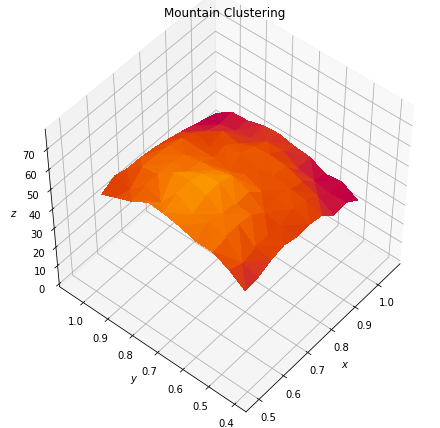
\includegraphics[scale = 0.45]{figures/iris/mountain-i.png}
    \caption{Initial mountain function for the mountain clustering using the euclidean norm.}
    \label{fig:mon-i-iris}
\end{figure}

\begin{figure}[ht]
    \centering
    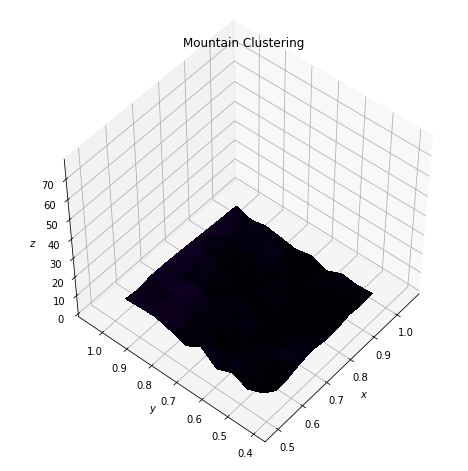
\includegraphics[scale = 0.45]{figures/iris/mountain-f.png}
    \caption{Final mountain function for the mountain clustering using the euclidean norm.}
    \label{fig:mon-f-iris}
\end{figure}

\begin{figure}[ht]
    \centering
    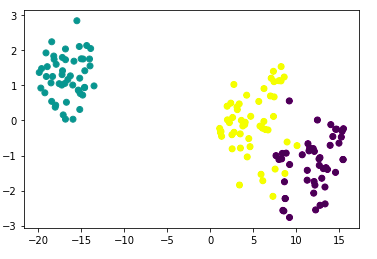
\includegraphics[scale = 0.45]{figures/iris/mountain.png}
    \caption{Clustering for the iris dataset using the mountain algorithm.}
    \label{fig:mon-iris}
\end{figure}


\subsection{Credit card dataset}
This dataset includes two classes, highly unbalanced: fraud or not fraud.
\subsubsection{Subtractive clustering}
    In Tables \ref{tab:c1_n_s}, \ref{tab:c2_n_s} and \ref{tab:ce_n_s} are shown the number of clusters found for the three datasets of credit card fraud. In this case, we observe that the cosine norm achieves 2 clusters, the expected ones. But probably more clusters are not a wrong performance, rather than a different form of viewing the data. We will refer then to the validation indices to see when the performance is better. Also, in Figure~\ref{fig:credit_s_i} is shown the initial density function for the credit card reduced dataset and $r_a = 0.5$, with the euclidean distance. Figure~\ref{fig:credit_s_f} shows the final state.
    \begin{table}[ht!]
        \centering
        \begin{tabular}{lrrr}
        \toprule
        $r_a$ &  euclidean &  cosine &  cityblock \\
        \midrule
        0.4 &         10 &       2 &         52 \\
        0.5 &          7 &       2 &         21 \\
        0.7 &          4 &       2 &          8 \\
        \bottomrule \\
        \end{tabular}
        \caption{Number of clusters found by the subtractive algorithm for the credit card dataset.}
        \label{tab:c1_n_s}
    \end{table}
    
    \begin{table}[ht!]
        \centering
        \begin{tabular}{lrrr}
        \toprule
        $r_a$ &  euclidean &  cosine &  cityblock \\
        \midrule
        0.4 &          8 &       2 &         23 \\
        0.5 &          5 &       2 &         11 \\
        0.7 &          3 &       2 &          5 \\
        \bottomrule \\
        \end{tabular}
        \caption{Number of clusters found by the subtractive algorithm for the credit card reduced dataset.}
        \label{tab:c2_n_s}
    \end{table}
    
    \begin{table}[ht!]
        \centering
        \begin{tabular}{lrrr}
        \toprule
        $r_a$ &  euclidean &  cosine &  cityblock \\
        \midrule
        0.4 &         99 &       8 &         99 \\
        0.5 &         99 &       7 &         99 \\
        0.7 &         99 &       4 &         99 \\
        \bottomrule \\
        \end{tabular}
        \caption{Number of clusters found by the subtractive algorithm for the credit card embbeded dataset.}
        \label{tab:ce_n_s}
    \end{table}
    
    The algorithm has an emergency stopping criteria, the number of iterations. Due to the fact that they are 100, is clear that for the euclidean distance in the embbeded dataset much more clusters are achieved. This may be due to the spatial distribution of the data, as shwon in the results of Figure~\ref{fig:credit_s}.
    
    \begin{table}[ht!]
        \centering
        \begin{tabular}{lrrr}
        \toprule
        $r_a$ &  euclidean &    cosine &  cityblock \\
        \midrule
        0.4 &   3.029305 &  0.981477 &   3.374885 \\
        0.5 &   3.441991 &  0.981142 &   3.349646 \\
        0.7 &   3.737428 &  0.981221 &   4.300733 \\
        \bottomrule \\
        \end{tabular}
        \caption{Davies Bouldin index for the credit card dataset clustered by the subtractive algorithm.}
        \label{tab:c1_db_s}
    \end{table}
    
    \begin{table}[ht!]
        \centering
        \begin{tabular}{lrrr}
        \toprule
        $r_a$ &     euclidean &         cosine &     cityblock \\
        \midrule
        0.4 &  34200.815670 &  181518.597459 &   4712.546985 \\
        0.5 &  45858.080636 &  181504.729539 &  10983.494778 \\
        0.7 &  67334.688094 &  181520.031384 &  30413.670844 \\
        \bottomrule \\
        \end{tabular}
        \caption{Calisnki-Harabsz score for the credit card dataset clustered by the subtractive algorithm.}
        \label{tab:c1_ch_s}
    \end{table}
    
    In Tables \ref{tab:c1_db_s} and \ref{tab:c1_db_s} are shown the results for the validation of the clustering in the original credit card dataset. We saw that, for the cosine metric the number of clusters found are the expected, and is actually revised by these scores, that classify this metric as the one that performs the better. \\
    
    \begin{table}[ht!]
        \centering
        \begin{tabular}{lrrr}
        \toprule
        $r_a$ &  euclidean &    cosine &  cityblock \\
        \midrule
        0.4 &   2.409494 &  0.875412 &   3.139200 \\
        0.5 &   2.088824 &  0.875412 &   2.601788 \\
        0.7 &   1.468652 &  0.875644 &   3.157173 \\
        \bottomrule \\
        \end{tabular}
        \caption{Davies Bouldin index for the credit card reduced dataset clustered by the subtractive algorithm.}
        \label{tab:c2_db_s}
    \end{table}
    
    \begin{table}[ht!]
        \centering
        \begin{tabular}{lrrr}
        \toprule
        $r_a$ &      euclidean &         cosine &     cityblock \\
        \midrule
        0.4 &   47725.987561 &  210512.707501 &  12023.907405 \\
        0.5 &   92681.517486 &  210512.707501 &  31914.695617 \\
        0.7 &  113693.471190 &  210511.841004 &  59832.246699 \\
        \bottomrule \\
        \end{tabular}
        \caption{Calisnki-Harabsz score for the reduced credit card dataset clustered by the subtractive algorithm.}
        \label{tab:c2_ch_s}
    \end{table}
    
    In Tables \ref{tab:c2_db_s} and \ref{tab:c2_ch_s} are shown the indices for the reduced dataset by PCA. Again, the performance shown by these corresponds to the fact that the cosine metric achieves the expected number of clusters.
    
    \begin{table}[ht!]
        \centering
        \begin{tabular}{lrrr}
        \toprule
        $r_a$ &  euclidean &    cosine &  cityblock \\
        \midrule
        0.4 &   1.080875 &  1.176533 &   1.253805 \\
        0.5 &   1.050448 &  1.093338 &   1.333077 \\
        0.7 &   0.953949 &  0.866116 &   1.043586 \\
        \bottomrule \\
        \end{tabular}
        \caption{Davies Bouldin index for the credit card embbeded dataset clustered by the subtractive algorithm.}
        \label{tab:ce_db_s}
    \end{table}
    
    \begin{table}[ht!]
        \centering
        \begin{tabular}{lrrr}
        \toprule
        $r_a$ &      euclidean &         cosine &      cityblock \\
        \midrule
        0.4 &   83056.373617 &  174368.043596 &   77677.563496 \\
        0.5 &  109156.916197 &  185793.584797 &   88929.724177 \\
        0.7 &  142020.902180 &  217192.867615 &  116444.149920 \\
        \bottomrule \\
        \end{tabular}
        \caption{Calisnki-Harabsz score for the reduced credit card dataset clustered by the subtractive algorithm.}
        \label{tab:ce_ch_s}
    \end{table}
    
    Finally, Tables \ref{tab:ce_db_s} and \ref{tab:ce_ch_s} are shown the validity indices or the embbeded dataset. These indices show a poor performance in all cases, reflecting the amount of clusters found by the algorithm in this particular dataset. Probably, the information given by the embbeding is not enough to show the full structure of the data.
    
    \begin{figure}[ht!]
        \centering
        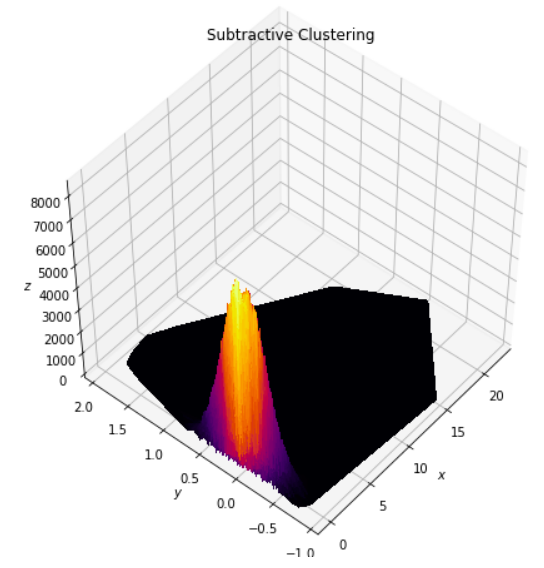
\includegraphics[scale = 0.4]{figures/credit/credit_s_i.png}
        \caption{Initial density function for the credit card dataset in the subtractive clustering algorithm.}
        \label{fig:credit_s_i}
    \end{figure}
    
    \begin{figure}[ht!]
        \centering
        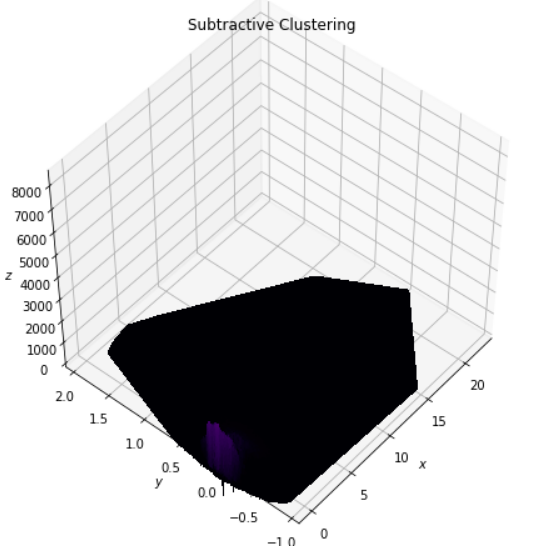
\includegraphics[scale = 0.4]{figures/credit/credit_s_f.png}
        \caption{Final density function for the credit card dataset in the subtractive clustering algorithm.}
        \label{fig:credit_s_f}
    \end{figure}
    
    \begin{figure}[ht!]
        \centering
        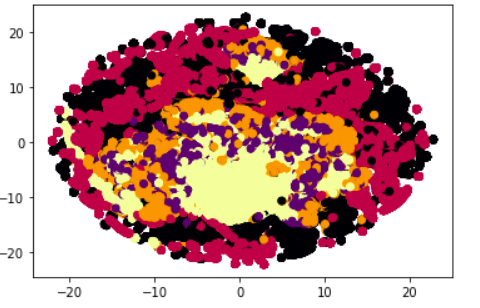
\includegraphics[scale = 0.4]{figures/credit/credit_s.png}
        \caption{Clustering for the credit card dataset in the subtractive clustering algorithm.}
        \label{fig:credit_s}
    \end{figure}
\subsubsection{Mountain clustering} Tables \ref{tab:c2_n_m} and \ref{tab:ce_n_m} show the number of clusters found by the mountain algorithm in the embbeded and reduced dataset, with variations in the smoothing paramenter $\sigma$ and the metric.

\begin{table}[ht!]
    \centering
   \begin{tabular}{lrrr}
    \toprule
    $\sigma$ &  euclidean &  cosine &  cityblock \\
    \midrule
    0.4 &          8 &       7 &          2 \\
    0.5 &          4 &       5 &          2 \\
    0.7 &          3 &       3 &          2 \\
    \bottomrule \\
    \end{tabular}
    \caption{Number of clusters found by the mountain algorithm in the reduced credit card dataset.}
    \label{tab:c2_n_m}
\end{table}

\begin{table}[ht!]
    \centering
    \begin{tabular}{lrrr}
    \toprule
    $\sigma$ &  euclidean &  cosine &  cityblock \\
    \midrule
    0.4 &         10 &       5 &          9 \\
    0.5 &          9 &       4 &         10 \\
    0.7 &          9 &       4 &          9 \\
    \bottomrule \\
    \end{tabular}
    \caption{Number of clusters found by the mountain algorithm in the embbeded credit card dataset.}
    \label{tab:ce_n_m}
\end{table}

In this case, we observe that the number of clusters is reduced in comparison with the subtractive algorithm, however, the metric that only finds the two existing clusters in the dataset is the manhattan, and only in the reduced one. The embbeded one, again, does not seem to provide enough information to perform a good clustering.

\begin{table}[ht!]
    \centering
    \begin{tabular}{lrrr}
        \toprule
        $\sigma$ &  euclidean &    cosine &  cityblock \\
        \midrule
        0.4 &   5.395964 &  2.539999 &   6.582867 \\
        0.5 &   5.076245 &  3.047503 &   6.582867 \\
        0.7 &   4.635804 &  1.861457 &   6.582867 \\
        \bottomrule \\
        \end{tabular}
    \caption{Davies Bouldin index for the reduced credit card dataset clustered by the mountain algorithm.}
    \label{tab:c2_db_m}
\end{table}

\begin{table}[ht!]
    \centering
    \begin{tabular}{lrrr}
    \toprule
    $\sigma$ &    euclidean &         cosine &    cityblock \\
    \midrule
    0.4 &  2612.705876 &   41225.158046 &  4029.893595 \\
    0.5 &  3689.213460 &   58473.394701 &  4029.893595 \\
    0.7 &  3966.374184 &  110716.512521 &  4029.893595 \\
    \bottomrule \\
    \end{tabular}
    \caption{Calinski-Harabasz score for the reduced credit card dataset clustered by the mountain algorithm.}
    \label{tab:c2_ch_m}
    \end{table}
    
    In Tables \ref{tab:c2_db_m} and \ref{tab:c2_ch_m} are shown the validity indices for the clustering in the reduced dataset.
    
\begin{table}[ht!]
    \centering
    \begin{tabular}{lrrr}
        \toprule
        $\sigma$ &  euclidean &    cosine &  cityblock \\
        \midrule
        0.4 &   0.891413 &  0.967157 &   0.946406 \\
        0.5 &   0.884992 &  0.878476 &   0.891413 \\
        0.7 &   0.884992 &  0.865683 &   0.884992 \\
        \bottomrule \\
        \end{tabular}
    \caption{Davies Bouldin index for the embbeded credit card dataset clustered by the mountain algorithm.}
    \label{tab:ce_db_m}
\end{table}

\begin{table}[ht!]
    \centering
    \begin{tabular}{lrrr}
        \toprule
        $\sigma$ &      euclidean &         cosine &      cityblock \\
        \midrule
        0.4 &  198415.832838 &  193511.849750 &  188520.438083 \\
        0.5 &  208251.768500 &  207307.628003 &  198415.832838 \\
        0.7 &  208251.768500 &  217172.104734 &  208251.768500 \\
        \bottomrule \\
        \end{tabular}
    \caption{Calinski-Harabasz score for the embbeded credit card dataset clustered by the mountain algorithm.}
    \label{tab:ce_ch_m}
\end{table}

\section{Conclusions}

\nocite{*}
\bibliography{ref}
\bibliographystyle{IEEEtran}


\end{document}
